\documentclass[10pt,landscape]{article}
\usepackage{multicol}
\usepackage{calc}
\usepackage{ifthen}
\usepackage[landscape, a4paper, top=3mm, left=3mm, right=3mm, bottom=3mm]{geometry}
\usepackage[
     pdftex,
     bookmarksopen=true,
     pdfauthor={Justin Iven Müller},
     pdftitle={Analysis 1 Cheatsheet},
     colorlinks=true,
     linkcolor=blue,
     urlcolor=blue
]{hyperref}
\usepackage{amsmath,amssymb,amsfonts}
\usepackage{enumitem}
\usepackage{tikz}
\usepackage{pgfplots}
\usepgfplotslibrary{fillbetween}
\usepackage{polynom}

\begin{document}
% Turn off header and footer
\pagestyle{empty}
 

% Redefine section commands to use less space
\makeatletter
\renewcommand{\section}{\@startsection{section}{1}{0mm}%
                                {-1ex plus -.5ex minus -.2ex}%
                                {0.5ex plus .2ex}%x
                                {\color{blue}\normalfont\large\bfseries}}
\renewcommand{\subsection}{\@startsection{subsection}{2}{0mm}%
                                {-1explus -.5ex minus -.2ex}%
                                {0.5ex plus .2ex}%
                                {\normalfont\normalsize\bfseries}}
\renewcommand{\subsubsection}{\@startsection{subsubsection}{3}{0mm}%
                                {-1ex plus -.5ex minus -.2ex}%
                                {1ex plus .2ex}%
                                {\normalfont\small\bfseries}}
\makeatother

% Remove indentation in itemize/enumerate and set left margin to zero
\setlist[itemize]{leftmargin=*}
\setlist[enumerate]{leftmargin=*}

% Don't print section numbers
\setcounter{secnumdepth}{0}

% Set font size and alignment for the whole document
\raggedright
\footnotesize

% Set column separation
% \setlength{\columnseprule}{1pt}
% \def\columnseprulecolor{\color{blue}}

\begin{multicols*}{4}

\begin{center}
     \Large{\textbf{Analysis 1}} \\
\end{center}

% 
\section{Funktionen}
Eine Funktion $f$ ordnet jedem Element $x$ aus einem Definitionsbereich $D$ genau einen Wert $f(x)$ zu.

\subsection*{Grundbegriffe}
\begin{itemize}
\item \textbf{Definitionsbereich $D$}: alle $x$, für die $f(x)$ definiert ist.
\item \textbf{Wertebereich $W$}: alle Werte $f(x)$, die tatsächlich auftreten.
\item \textbf{Graph}: Menge aller Punkte $(x,f(x))$ im Koordinatensystem.
\end{itemize}

\subsection*{Wichtige Eigenschaften}
\textbf{Gerade Funktion}: $f(-x)=f(x)$. Graph ist symmetrisch zur $y$-Achse.  
\textbf{Ungerade Funktion}: $f(-x)=-f(x)$. Graph ist punktsymmetrisch zum Ursprung.

\subsection*{Umkehrfunktionen}
$f$ besitzt eine Umkehrfunktion $f^{-1}$ genau dann, wenn $f$ \textbf{injektiv} ist.  
\[
(f^{-1})'(y)=\frac{1}{f'(x)}\quad\text{mit }y=f(x).
\]
\textit{Erklärung: Eine Umkehrfunktion ``dreht'' die Zuordnung um; ihre Steigung ist der Kehrwert der ursprünglichen.}

\section{Polynome und Algebraische Werkzeuge}
Ein Polynom vom Grad $n$ hat höchstens $n$ Nullstellen.

\subsection*{Horner-Schema}
Effiziente Berechnung von $f(x_0)$ und Polynomdivision durch $(x-x_0)$.

\subsection*{Zerlegungssatz}
Hat $f(x_0)=0$, so lässt sich schreiben:
\[
f(x) = (x-x_0)\cdot q(x).
\]

\subsection*{Wichtige Summenformeln}
\[
\sum_{k=1}^n k = \frac{n(n+1)}{2},\qquad
\sum_{k=1}^n k^2 = \frac{n(n+1)(2n+1)}{6}.
\]

\textit{Erklärung: Diese Formeln ermöglichen es, Summen geschlossener auszudrücken.}

\section{Differentialrechnung}
\subsection*{Definition der Ableitung}
\[
f'(x)=\lim_{h\to0}\frac{f(x+h)-f(x)}{h}.
\]

\textit{Interpretation: $f'(x)$ beschreibt die Steigung der Tangente an den Graphen an der Stelle $x$.}

\subsection*{Ableitungsregeln}
Linearität:
\[
(c\cdot f)' = c\cdot f', \quad (f+g)' = f'+g'
\]

Produktregel:
\[
(fg)' = f'g + fg'
\]

Quotientenregel:
\[
\left(\frac{u}{v}\right)' = \frac{u'v-uv'}{v^2}
\]

Kettenregel (Zusammensetzung $F(u(x))$):
\[
(F\circ u)' = F'(u(x)) \cdot u'(x)
\]

\subsection*{Tangente}
\[
T(x)=f(x_0)+f'(x_0)(x-x_0).
\]

\textit{Bedeutung: Lokale lineare Annäherung an den Graphen.}

\subsection*{Extremstellen (Hoch-/Tiefpunkte)}
\[
f'(x_0)=0.
\]
Zur Klassifikation:
\[
\begin{cases}
f''(x_0) > 0 & \text{Minimum}\\
f''(x_0) < 0 & \text{Maximum}\\
f''(x_0) = 0 & \text{keine eindeutige Aussage}
\end{cases}
\]

\section{Integralrechnung}
\subsection*{Definition als Grenzwert}
\[
\int_a^b f(x)\,dx = \lim_{n\to\infty}\sum_{k=1}^n f(x_k)\Delta x.
\]

\textit{Interpretation: Fläche unter dem Graphen zwischen $a$ und $b$.}

\subsection*{Hauptsatz der Differential- und Integralrechnung}
Ist $F$ eine Stammfunktion von $f$, dann:
\[
\int_a^b f(x)\,dx = F(b)-F(a).
\]

\subsection*{Wichtige Integrationsregeln}
Lineare Operationen:
\[
\int(c\cdot f)dx=c\cdot\int f dx,\qquad \int(f+g)dx=\int f dx + \int g dx.
\]

Potenzregel ($n\neq -1$):
\[
\int x^n dx = \frac{x^{n+1}}{n+1} + C.
\]

Substitution:
\[
\int f(u(x))u'(x)\,dx = \int f(u)\,du.
\]

\section{Folgen und Reihen}
\subsection*{Grenzwert einer Folge}
Eine Folge $(a_n)$ konvergiert gegen $L$, wenn:
\[
\lim_{n\to\infty} a_n = L.
\]

\textit{Bedeutung: Für grosse $n$ wird $a_n$ beliebig nahe an $L$.}

\subsection*{Reihen}
Eine Reihe ist die Summe einer Folge:
\[
\sum_{n=1}^{\infty} a_n.
\]

\textbf{Geometrische Reihe:}
\[
\sum_{k=0}^\infty q^k = \frac{1}{1-q} \quad \text{für } |q|<1.
\]

\section{Grenzwerte und Stetigkeit}
\[
\lim_{x\to x_0} f(x)=f(x_0) \quad\Rightarrow\quad f \text{ ist stetig in } x_0.
\]

\textit{Bedeutung: Keine Sprungstellen; Graph kann ohne Absetzen gezeichnet werden.}

\section{Basics}

\subsection{Intervalle}
\begin{itemize}
    \item Offenes Intervall: \(]a,b[ \ = (a,b) = \{ x \in \mathbb{R} \mid a < x < b \}\)
    \item Geschlossenes Intervall: \([a,b] = \{ x \in \mathbb{R} \mid a \leq x \leq b \}\)
    \item Halboffenes Intervall: \([a,b[ = \{ x \in \mathbb{R} \mid a \leq x < b \}\), \(]a,b] = \{ x \in \mathbb{R} \mid a < x \leq b \}\)
    \item Unendliche Intervalle: \((-\infty, a] = \{ x \in \mathbb{R} \mid x \leq a \}\), \([b, \infty) = \{ x \in \mathbb{R} \mid x \geq b \}\)
\end{itemize}

\subsection{Quadratische Gleichungen}
Eine quadratische Gleichung hat die Form \(ax^2 + bx + c = 0\) mit \(a \neq 0\).

\subsubsection{Lösungsformel}
Die Lösungen sind gegeben durch:
\[
x_{1,2} = \frac{-b \pm \sqrt{b^2 - 4ac}}{2a}.
\]

\subsubsection{Diskriminante}
Die Diskriminante \(D = b^2 - 4ac\) entscheidet über die Art der Lösungen:
\begin{itemize}
    \item \(D > 0\): zwei verschiedene reelle Lösungen
    \item \(D = 0\): eine doppelte reelle Lösung
    \item \(D < 0\): keine reellen Lösungen (komplexe Lösungen)
\end{itemize}

\subsection{Potenzregel}
\begin{align*}
    a^m \cdot a^n &= a^{m+n} \\
    \frac{a^m}{a^n} &= a^{m-n} \\
    (a^m)^n &= a^{m \cdot n} \\
    a^0 &= 1 \quad (a \neq 0) \\
    a^{-n} &= \frac{1}{a^n} \quad (a \neq 0) \\
    (ab)^n &= a^n b^n \\
    \left(\frac{a}{b}\right)^n &= \frac{a^n}{b^n} \quad (b \neq 0) \\
    a^{\frac{m}{n}} &= \sqrt[n]{a^m} = (\sqrt[n]{a})^m \quad (n \neq 0)
\end{align*}

\subsection{Logarithmusregeln}
\begin{align*}
    \log_a(xy) &= \log_a(x) + \log_a(y) \\
    \log_a\left(\frac{x}{y}\right) &= \log_a(x) - \log_a(y) \\
    \log_a(x^r) &= r \cdot \log_a(x) \\
    \log_a(1) &= 0 \\
    \log_a(a) &= 1 \\
    \log_a(x) &= \frac{\log_b(x)}{\log_b(a)} \quad (a, b > 0, \; a, b \neq 1)
\end{align*}

\subsection{Binomische Formeln}
\begin{align*}
    (a + b)^2 &= a^2 + 2ab + b^2 \\
    (a - b)^2 &= a^2 - 2ab + b^2 \\
    (a + b)(a - b) &= a^2 - b^2
\end{align*}

\subsection{Fakultät}
Die Fakultät einer natürlichen Zahl \(n\) ist definiert als:
\[
n! = n \cdot (n-1) \cdot (n-2) \cdots 2 \cdot 1,
\]mit der Besonderheit \(0! = 1\).

\subsection{Binomialkoeffizient}
Der Binomialkoeffizient \(\binom{n}{k}\) gibt die
Anzahl der Möglichkeiten an, \(k\) Objekte aus \(n\) auszuwählen, und ist definiert als:
\[\binom{n}{k} = \frac{n!}{k!(n-k)!} \quad \text{für } 0 \leq k \leq n.\]

\subsection{Summenregeln}
Für endliche Summen gelten folgende Regeln:
\begin{align*}
    \sum_{i=1}^{n} c &= n \cdot c \\
    \sum_{i=1}^{n} (a_i + b_i) &= \sum_{i=1}^{n} a_i + \sum_{i=1}^{n} b_i \\
    \sum_{i=1}^{n} (c \cdot a_i) &= c \cdot \sum_{i=1}^{n} a_i
\end{align*}

\subsection{Betragsfunktion}
Der Betrag einer reellen Zahl \(x\) ist definiert als:
\[|x| = 
\begin{cases}
x, & \text{falls } x \geq 0 \\
-x, & \text{falls } x < 0
\end{cases}\]

\section{Funktionen}
Eine \emph{Funktion} \(f\) von der Menge \(A\) nach \(B\) ist eine Relation, die \emph{linksvollständig} und \emph{rechtseindeutig} ist. Man schreibt:
\[
f: A \to B,
\]
und für jedes \(x\in A\) existiert genau ein \(y\in B\) mit \(y=f(x)\).

\subsection{Schreibweise}
Oft werden Funktionen durch Angabe von Definitions- und Zielmenge sowie einer
Zuordnungsvorschrift beschrieben. Beispielsweise gilt:
\[
f = \bigl(\{(x, x^3) \mid x \in \mathbb{N}\}, \mathbb{N}, \mathbb{N}\bigr)
\]
bzw. äquivalent in der gebräuchlicheren Schreibweise:
\[
f : \mathbb{N} \to \mathbb{N}, \quad f(x) = x^3.
\]

\subsection{Injektive Funktionen}
Eine Funktion $f : A \to B$ ist \emph{injektiv}, falls die Relation \emph{linksvollständig}, \emph{rechtseindeutig} und zusätzlich \emph{linkseindeutig} ist:
\begin{align*}
  \forall x_1, x_2 &\in A (f(x_1) = f(x_2) \Rightarrow x_1 = x_2)\\
  \forall x_1, x_2 &\in A (x_1 \neq x_2 \Rightarrow f(x_1) \neq f(x_2))
\end{align*}
Jedes Element in \(A\) wird auf ein eigenes unterschiedliches Element in \(B\) abgebildet.

Notation: $f : A \hookrightarrow B$.

\subsection{Umkehrbarkeit}
Eine Funktion $f : A \to B$ ist genau dann \emph{umkehrbar}, wenn sie injektiv ist. Dann gilt:
\[
f^{-1} : \operatorname{im}(f) \to A.
\]
\[
(G^\prime_f, \operatorname{im}(f), A), \quad G^\prime_f = \{(y,x) | (x,y) \in G_f\}
\]

\subsection{Surjektivität}
Eine Funktion $f : A \to B$ ist \emph{surjektiv}, falls die Relation \emph{linksvollständig}, \emph{rechtseindeutig} und zusätzlich \emph{rechtsvollständig} ist:
\[
\operatorname{im}(f) = B
\]
Jedes Element in \(B\) wird von mindestens einem Element in \(A\) erreicht.\\
Notation: \(f:A \twoheadrightarrow B\)

\subsection{Bijektivität}
Eine Funktion $f : A \to B$ ist \emph{bijektiv}, wenn sie sowohl injektiv als auch surjektiv ist. Die Umkehrfunktion ist dann definiert durch:
\[
f^{-1} : B \to A.
\]
J
Notation: \(f : A \rightleftharpoons B\)


\subsection{Umkehrfunktion}
Für eine bijektive Funktion $f : A \rightleftharpoons B$ gilt:
\[
f^{-1} \circ f = \operatorname{id}_A, \qquad f \circ f^{-1} = \operatorname{id}_B.
\]

\subsection{Komposition}
Für $g : A \to B$ und $f : B \to C$ definiert man die \emph{Komposition}:
\[
(f \circ g)(x) = f(g(x)), \quad f \circ g : A \to C.
\]
Komposition ist \emph{assoziativ}:
\[
h \circ (g \circ f) = (h \circ g) \circ f.
\]

\subsection{Eigenschaften der Komposition}
Für Funktionen $f : A \to B$ und $g : B \to C$ gilt:
\begin{itemize}
  \item Sind $f$ und $g$ injektiv, dann ist $g \circ f$ injektiv.
  \item Sind $f$ und $g$ surjektiv, dann ist $g \circ f$ surjektiv.
  \item Sind $f$ und $g$ bijektiv, dann ist $g \circ f$ bijektiv.
\end{itemize}


\section{Polynomfunktionen}
Ein Polynom ist eine Funktion der Form
\[
    f(x) = a_n x^n + a_{n-1} x^{n-1} + \ldots + a_1 x + a_0
\]
mit $a_n, a_{n-1}, \ldots, a_1, a_0 \in \mathbb{R}$ und $a_n \neq 0$.
Der höchste Exponent $n$ heisst \emph{Grad} des Polynoms.

\subsection{Horner-Schema}
Das Horner-Schema ist eine effiziente Methode zur Auswertung von Polynomen. Es hat die Form:
\[
    f(x) = (((a_n x + a_{n-1}) x + a_{n-2}) x + \ldots + a_1) x + a_0
\]

Linearfaktorisierung eines Polynoms nach dem Horner-Schema:
\[
    f(x) = 2x^3-12x^2+22x-12
\]

\begin{center}
  \polyhornerscheme[x=2, showvar=true, stage=8, tutor=true, tutorlimit=8, tutorstyle=\color{lightgray}]{2x^3-12x^2+22x-12}
\end{center}
\[
    f(x) = (2x^2 - 8x + 6)(x - 2)
\]

\subsection{Nullstellen von Polynomen}
Ein Polynom von Grad \(n\) hat höchstens \(n\) reelle Nullstellen.

\subsection{\(m\)-fache Nullstelle}
\(x_0\) ist eine \(m\)-fache Nullstelle des Polynoms \(f(x)\), wenn \(f(x)\) in der Form
\[
    f(x) = (x - x_0)^m \cdot g(x)
\]
geschrieben werden kann, wobei \(g(x)\) ein Polynom ist, das \(x_0\) nicht als Nullstelle hat.

\subsection{Polynomdivision}
Mit dem Horner-Schema können nur Linearfaktoren \((x - x_0)\) abgeteilt werden. Für die Division durch Polynome höheren Grades wird die Polynomdivision verwendet:
\[
    f(x) = g(x) \cdot Q(x) + R(x)
\]
wobei \(Q(x)\) der Quotient und \(R(x)\) der Rest ist. Der Grad des Rests ist kleiner als der Grad des Divisors \(g(x)\).
\begin{center}
    \tiny
    \polylongdiv[style=C, div=:]{x^3-6x^2+11x-6}{x^2+x-4}
\end{center}
\section{Rationale Funktionen}
Eine rationale Funktion ist eine Funktion der Form
\[
    f(x) = \frac{p(x)}{q(x)} = \frac{a_n x^n + a_{n-1} x^{n-1} + \ldots + a_1 x + a_0}{b_m x^m + b_{m-1} x^{m-1} + \ldots + b_1 x + b_0}
\]
wobei \(p(x)\) und \(q(x)\) Polynome sind und \(q(x) \neq 0\).

\subsection{Eigenschaften}
Rationale Funktionen haben folgende Eigenschaften:
\begin{itemize}
    \item Sie sind definiert, solange der Nenner \(q(x)\) nicht null ist.
    \item Sie können durch Partialbruchzerlegung in einfachere Brüche zerlegt werden.
    \item Sie haben höchstens so viele Nullstellen wie der Grad des Zählers.
\end{itemize}

\subsection{Definitionslücken}
Rationale Funktionen können Definitionslücken aufweisen, die auftreten, wenn der Nenner \(q(x)\) an bestimmten Stellen null wird. An diesen Stellen ist die Funktion nicht definiert.

Sei \(x_0\) eine Definitionslücken von \(f(x)\). Der Linearfaktor \((x - x_0)\) sei aus \(p(x)\) und \(q(x)\) abgeteilt:
\[
    f(x) = \frac{(x - x_0)^{j_p} \cdot p_1(x)}{(x - x_0)^{j_q} \cdot q_1(x)}, \quad p_1(x_0), \quad q_1(x_0) \neq 0
\]
mit \(j_p, j_q \in \mathbb{N}\) und \(j_q > 1\).

\begin{itemize}
    \item Wenn \(j_p \le j_q\), dann ist \(x_0\) eine \emph{hebbare} Definitionslücke.
    \item Wenn \(j_p < j_q\), dann ist \(x_0\) eine Polstelle der Ordnung \(j_q - j_p\).
    \begin{itemize}
        \item Ordnung gerade: Polstelle ohne Vorzeichenwechsel.
        \item Ordnung ungerade: Polstelle mit Vorzeichenwechsel.
    \end{itemize}
    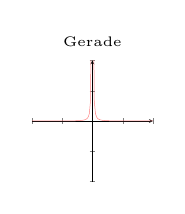
\begin{tikzpicture}[scale=.45]
        \begin{axis}[axis lines=middle, xmin=-2, xmax=2, ymin=-2, ymax=2, width=5cm, height=5cm, yticklabel={\empty}, xticklabel={\empty}]
            \addplot[domain=-2:2, samples=100, red!50] {1/(20*x)^2};
        \end{axis}
      \node[anchor=south] at (current bounding box.north) {\tiny{Gerade}};
    \end{tikzpicture}
    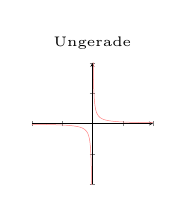
\begin{tikzpicture}[scale=.45]
        \begin{axis}[axis lines=middle, xmin=-2, xmax=2, ymin=-2, ymax=2, width=5cm, height=5cm, yticklabel={\empty}, xticklabel={\empty}]
            \addplot[domain=-2:0, samples=100, red!50] {1/(20*x)};
            \addplot[domain=0:2, samples=100, red!50] {1/(20*x)};
        \end{axis}
      \node[anchor=south] at (current bounding box.north) {\tiny{Ungerade}};
    \end{tikzpicture}
    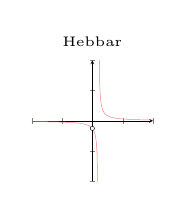
\begin{tikzpicture}[scale=.45]
        \begin{axis}[axis lines=middle, xmin=-2, xmax=2, ymin=-2, ymax=2, width=5cm, height=5cm, yticklabel={\empty}, xticklabel={\empty}]
            \addplot[domain=-2:0.2, samples=100, red!50] {x/(20*x*(x-0.2))};
            \addplot[domain=0.2:2, samples=100, red!50] {x/(20*x*(x-0.2))};
                \node at (axis cs:0,-0.25) [circle, draw=black, fill=white, inner sep=1.2pt] {};
        \end{axis}
      \node[anchor=south] at (current bounding box.north) {\tiny{Hebbar}};
    \end{tikzpicture}
\end{itemize}

\subsection{Asymptoten}
Rationale Funktionen können folgende Asymptoten haben:
\begin{itemize}
    \item \emph{Vertikale Asymptoten}: Treten auf, wenn \(q(x) = 0\) und \(p(x) \neq 0\).
    \item \emph{Horizontale Asymptoten}: Bestimmen das Verhalten von \(f(x)\) für \(x \to \pm \infty\).
    \item \emph{Polynomiale Asymptoten}: Treten auf, wenn der Grad des Zählers grösser ist als der Grad des Nenners. Sie können durch Polynomdivision gefunden werden.
\end{itemize}

\subsection{Graphen}
Der Graph einer rationalen Funktion kann durch Nullstellen und Asymptoten skizziert werden. Dabei sind die Nullstellen die Lösungen von \(p(x) = 0\) und die Asymptoten die Lösungen von \(q(x) = 0\).
\section{Differentialrechnung}
Sei \(f(x) : D \to \mathbb{R}\) eine Funktion. Die Ableitung \(f'(x_0)\) beschreibt die Änderungsrate der Funktion an der Stelle \(x_0\). Sie wird definiert als der Grenzwert des Differenzenquotienten:
\[
    f'(x_0) = \lim_{\Delta x \to 0} \frac{f(x_0 + \Delta x) - f(x_0)}{\Delta x} = \lim_{x \to 0} \frac{\Delta f}{\Delta x}(x_0) 
\]
\begin{center}
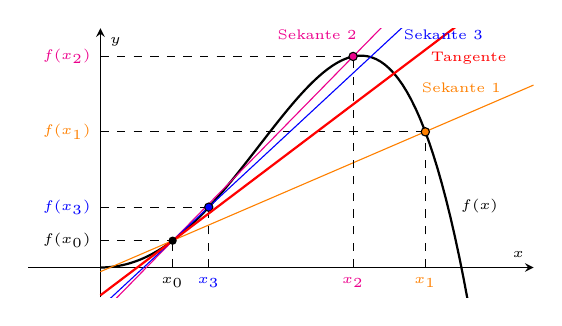
\begin{tikzpicture}[font=\tiny]
    \pgfplotsset{ticks=none}
    \begin{axis}
        [axis lines = middle,
        xlabel = \(x\),
        ylabel = \(y\),
        samples=100,
        ymin=-0.1, ymax=0.8,
        xmin=-0.2, xmax=1.2,
        width=8cm,
        height=5cm
        ]
        \node[above] at (axis cs:1.05,0.15) {\(f(x)\)};
        \addplot[domain=0:1.2, thick] { -4*x^4+2*x^3+2*x^2 };

        \draw[dashed, thin] (axis cs:0.9,0) node[below, orange] {$x_1$} -- (axis cs:0.9, { -4*0.9^4+2*0.9^3+2*0.9^2 });
        \draw[dashed, thin] (axis cs:0,{ -4*0.9^4+2*0.9^3+2*0.9^2 }) node[left, orange] {$f(x_1)$} -- (axis cs:0.9, { -4*0.9^4+2*0.9^3+2*0.9^2 });
        \addplot[domain=0:1.2, thin, orange] {0.520*x -0.014};
        \fill[draw=black, fill=orange] (axis cs:0.9, { -4*0.9^4+2*0.9^3+2*0.9^2 }) circle(1.5pt);
        
        \draw[dashed, thin] (axis cs:0.70,0) node[below, magenta] {$x_2$} -- (axis cs:0.70, { -4*0.70^4+2*0.70^3+2*0.70^2 });
        \draw[dashed] (axis cs:0,{ -4*0.70^4+2*0.70^3+2*0.70^2 }) node[left, magenta] {$f(x_2)$} -- (axis cs:0.70, { -4*0.70^4+2*0.70^3+2*0.70^2 });
        \addplot[domain=0:1.2, thin, magenta] {1.232*x -0.157};
        \fill[draw=black, fill=magenta] (axis cs:0.70, { -4*0.70^4+2*0.70^3+2*0.70^2 }) circle(1.5pt);
        
        \draw[dashed, thin] (axis cs:0.3,0) node[below, blue] {$x_3$} -- (axis cs:0.3, { -4*0.3^4+2*0.3^3+2*0.3^2 });
        \draw[dashed] (axis cs:0,{ -4*0.3^4+2*0.3^3+2*0.3^2 }) node[left, blue] {$f(x_3)$} -- (axis cs:0.3, { -4*0.3^4+2*0.3^3+2*0.3^2 });
        \addplot[domain=0:1.2, thin, blue] {1.120*x -0.134};
        \fill[draw=black, fill=blue] (axis cs:0.3, { -4*0.3^4+2*0.3^3+2*0.3^2 }) circle(1.5pt);
        
        \draw[dashed, thin] (axis cs:0.2,0) node[below] {$x_0$} -- (axis cs:0.2, { -4*0.2^4+2*0.2^3+2*0.2^2 });
        \draw[dashed, thin] (axis cs:0,{ -4*0.2^4+2*0.2^3+2*0.2^2 }) node[left] {$f(x_0)$} -- (axis cs:0.2, { -4*0.2^4+2*0.2^3+2*0.2^2 });
        \addplot[domain=0:1.2, thick, red] {0.912*x -0.093};
        \fill[black] (axis cs:0.2,{ -4*0.2^4+2*0.2^3+2*0.2^2 }) circle(1.5pt);
        
        \node[red] at (axis cs:1.02,0.7) {Tangente};
        \node[orange] at (axis cs:1,0.6) {Sekante 1};
        \node[magenta] at (axis cs:0.6,0.78) {Sekante 2};
        \node[blue] at (axis cs:0.95,0.78) {Sekante 3};
    \end{axis}
\end{tikzpicture}
\end{center}
    
\subsection{Ableitungsregeln}
\begin{itemize}
    \item \textbf{Faktorregel:} \((c \cdot f)'(x) = c \cdot f'(x)\)
    \item \textbf{Summenregel:} \((f + g)'(x) = f'(x) + g'(x)\)
    \item \textbf{Produktregel:} \((f \cdot g)'(x) = f'(x) \cdot g(x) + f(x) \cdot g'(x)\)
    \item \textbf{Quotientenregel:} \(\left(\frac{f}{g}\right)'(x) = \frac{f'(x) \cdot g(x) - f(x) \cdot g'(x)}{(g(x))^2}\)
    \item \textbf{Kettenregel:} \((f \circ g)'(x) = f'(g(x)) \cdot g'(x)\)
\end{itemize}

\subsection{Wichtige Ableitungen}
\begin{align*}
    (x^n)' &= n \cdot x^{n-1} \quad\text{ für } n \in \mathbb{R} \\
    (e^x)' &= e^x \\
    (\ln x)' &= \frac{1}{x} \quad \text{ für } x > 0 \\
    (\log_a x)' &= \frac{1}{x \ln a} \quad \text{ für } x > 0, a > 0, a \neq 1 \\
    (\sin x)' &= \cos x \\
    (\cos x)' &= -\sin x \\
\end{align*}

\subsection{Differenzierbarkeit}
Eine Funktion \(f(x)\) ist an der Stelle \(x_0\) differenzierbar, wenn die links- und rechtsseitigen Ableitungen übereinstimmen. Differenzierbarkeit impliziert Stetigkeit, aber nicht umgekehrt.\\
\emph{Definition:} Eine Funktion heisst differenzierbar, wenn die Ableitung an jeder Stelle ihres Definitionsbereichs existiert.

\subsection{Tangenten- und Normalengleichung}
Die Tangente an die Funktion \(f(x)\) an der Stelle \(x_0\) hat die Gleichung:
\[
    y = f'(x_0)(x - x_0) + f(x_0)
\]
Die Normalenlinie, die senkrecht zur Tangente steht, hat die Gleichung:
\[
    y = -\frac{1}{f'(x_0)}(x - x_0) + f(x_0)
\]

\subsection{Newton-Verfahren}
Das Newton-Verfahren ist ein iteratives Verfahren zur Bestimmung von Nullstellen einer Funktion. Gegeben sei eine Funktion \(f(x)\) und eine Näherung \(x_0\) für eine Nullstelle (Fixpunkt). Die Iterationsformel lautet:
\[
    x_{n+1} = x_n - \frac{f(x_n)}{f'(x_n)}
\]
Die Konvergenz des Verfahrens hängt von der Wahl der Startnäherung und den Eigenschaften der Funktion ab.


\section{Integralrechnung}
\subsection{Unbestimmte Integrale}
Sei \(f:\mathbb{R}\to\mathbb{R}\) eine Funktion.
Das \textbf{unbestimmte Integral} von \(f\) ist definiert als
\[\int f(x)\,dx = F(x) + C,
\]
wobei \(F\) eine Stammfunktion von \(f\) ist, also \(F'(x) = f(x)\) für alle \(x \in \mathbb{R}\), und \(C\) eine Konstante ist.

\subsection{Bestimmte Integrale}
Sei \(f:[a,b]\to\mathbb{R}\) eine Funktion.
Das \textbf{bestimmte Integral} von \(f\) über das Intervall \([a,b]\) ist definiert als
\[\int_a^b f(x)\,dx = F(b) - F(a),
\]
wobei \(F\) eine beliebige Stammfunktion von \(f\) ist, also \(F'(x) = f(x)\) für alle \(x \in [a,b]\).
\begin{center}
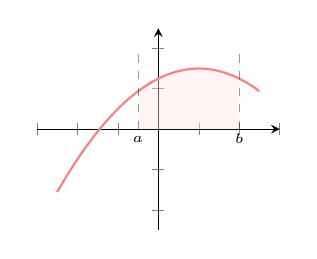
\begin{tikzpicture}
\begin{axis}[
    axis lines=middle,
    xmin=-3, xmax=3,
    ymin=-10, ymax=10,
    xtick distance=1, ytick distance=4,
    scale=.45, yticklabel={\empty}, xticklabel={\empty}
    ]
    \path [name path=xaxis] (axis cs:-10,0) -- (axis cs:10,0);
    \addplot [domain=-2.5:2.5, samples=100, name path=f, thick, color=red!50]{-x^2 + 2*x + 5};
    \addplot[red!10, opacity=0.4] fill between[of=f and xaxis, soft clip={domain=-0.5:2}];
    \draw [dashed, opacity=0.4] (axis cs:{-0.5,0}) -- (axis cs:{-0.5,8});
    \draw [dashed, opacity=0.4] (axis cs:{2,0}) -- (axis cs:{2,8});
    \node at (axis cs: -0.5,-1) {\tiny$a$};
    \node at (axis cs: 2,-1) {\tiny$b$};
\end{axis}
\end{tikzpicture}
\end{center}

\subsection{Flächeninhalt unter einer Funktion}
Sei \(f:[a,b]\to\mathbb{R}\) eine Funktion mit \(f(x) \geq 0\) für alle \(x \in [a,b]\).
Der Flächeninhalt \(A\) unter der Funktion \(f\) über das Intervall \([a,b]\) ist definiert als
\[A = \int_a^b f(x)\,dx.
\]

Für den Fall, dass \(f(x) \leq 0\) für alle \(x \in [a,b]\), ist der Flächeninhalt \(A\) über der Funktion \(f\) definiert als
\[A = -\int_a^b f(x)\,dx.
\]

\emph{Im Allgemeinen:} Sei \(X\) die Menge aller Nullstellen von \(f\) im Intervall \([a,b]\), also \(X = \{x_1, x_2, \ldots, x_n\}\) mit \(a = x_0 < x_1 < \ldots < x_n = b\).
Dann ist der Flächeninhalt \(A\) zwischen der Funktion \(f\) und der \(x\)-Achse über das Intervall \([a,b]\) definiert als
\[A = \sum_{i=0}^{n-1} \left| \int_{x_i}^{x_{i+1}} f(x)\,dx \right|.\]
\begin{center}
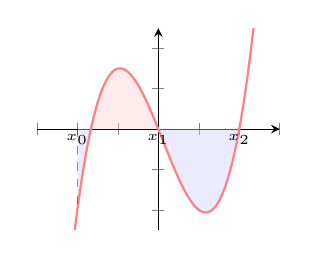
\begin{tikzpicture}
\begin{axis}[
    axis lines=middle,
    xmin=-3, xmax=3,
    ymin=-10, ymax=10,
    xtick distance=1, ytick distance=4,
    scale=.45, yticklabel={\empty}, xticklabel={\empty}
    ]
    \addplot [domain=-2.5:2.5, samples=100, name path=f, thick, color=red!50]{3*x^3 - x^2 - 10*x};
    \path [name path=xaxis] (axis cs:-10,0) -- (axis cs:10,0);
    \draw [dashed, opacity=0.4] (axis cs:{-2,0}) -- (axis cs:{-2,-8});
    \addplot[red!10, opacity=0.4] fill between [
        of=f and xaxis, soft clip={domain=-2:2},
        split,
        every even segment/.style = {blue!20!white},
        every odd segment/.style ={red!20!white}];
    \node at (axis cs: -2,-1) {\tiny$x_0$};
    \node at (axis cs: 0,-1) {\tiny$x_1$};
    \node at (axis cs: 2,-1) {\tiny$x_2$};

\end{axis}
\end{tikzpicture}
\end{center}




\subsection{Integral zwischen zwei Funktionen}
Seien \(f,g:[a,b]\to\mathbb{R}\) zwei Funktionen.
Das \textbf{Integral zwischen zwei Funktionen} \(f\) und \(g\) über das Intervall \([a,b]\) ist definiert als
\[\int_a^b (f(x) - g(x))\,dx = F(b) - G(a),
\]
wobei \(F\) eine Stammfunktion von \(f\) und \(G\) eine Stammfunktion von \(g\) ist.

\begin{center}
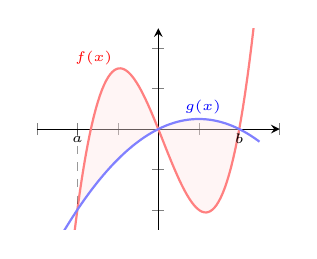
\begin{tikzpicture}
\begin{axis}[
    axis lines=middle,
    xmin=-3, xmax=3,
    ymin=-10, ymax=10,
    xtick distance=1, ytick distance=4,
    scale=.45, yticklabel={\empty}, xticklabel={\empty}
    ]
    \addplot [domain=-2.5:2.5, samples=100, name path=f, thick, color=red!50]{3*x^3 - x^2 - 10*x};
    \addplot [domain=-2.5:2.5, samples=100, name path=g, thick, color=blue!50]{- x^2 + 2*x};
    \addplot[red!10, opacity=0.4] fill between[of=f and g, soft clip={domain=-2:2}];
    \draw [dashed, opacity=0.4] (axis cs:{-2,0}) -- (axis cs:{-2,-8});
    \node[color=red, font=\footnotesize] at (axis cs: -1.6,7) {\tiny$f(x)$};
    \node[color=blue, font=\footnotesize] at (axis cs: 1.1,2.2) {\tiny$g(x)$};
    \node at (axis cs: -2,-1) {\tiny$a$};
    \node at (axis cs: 2,-1) {\tiny$b$};
\end{axis}
\end{tikzpicture}
\end{center}

\subsection{Integrationsregeln}
\subsubsection{Konstantenregel}
Sei \(c \in \mathbb{R}\) eine Konstante. Dann gilt für das Integral einer konstanten Funktion
\[\int_a^b c\,dx = c \cdot (b-a).\]

\subsubsection{Summenregel}
Seien \(f,g:[a,b]\to\mathbb{R}\) zwei Funktionen. Dann gilt für das Integral der Summe von zwei Funktionen
\[\int_a^b (f(x) + g(x))\,dx = \int_a^b f(x)\,dx + \int_a^b g(x)\,dx.\]

\subsubsection{Polynomregel}
Sei \(n \in \mathbb{N}_0\). Dann gilt für das Integral einer Potenzfunktion
\[\int x^n\,dx = \frac{1}{n+1} x^{n+1} + C.\]

\subsection{Integrale von ausgewählten Funktionen}
Potentz- und Logarithmusfunktionen:
\begin{align*}
\int a^x\,dx &= \frac{a^x}{\ln(a)} + C \quad (a > 0, a \neq 1)\\
\int \ln(x)\,dx &= x \ln(x) - x + C \quad (x > 0)\\
\int \log_a(x)\,dx &= \frac{x \ln(x) - x}{\ln(a)} + C \quad (a > 0, a \neq 1, x > 0)
\end{align*}
Trigonometrische Funktionen:
\begin{align*}
\int \sin(x)\,dx &= -\cos(x) + C\\
\int \cos(x)\,dx &= \sin(x) + C\\
\int \tan(x)\,dx &= -\ln|\cos(x)| + C
\end{align*}
\section{Folgen und Reihen}
Eine \textit{Folge} ist eine Abbildung, die jeder natürlichen Zahl \(n\) ein Element \(a_n\) aus einer Menge \(M\) zuordnet. Man schreibt eine Folge als  \(a = (a_n)\).\\
Eine \textit{Reihe} ist die Summe der Glieder einer Folge, dargestellt als \(\sum_{n=1}^{\infty} a_n\).

\subsection{Darstellung von Folgen}
Jedes Glied der Folge wird in der...
\begin{itemize}
    \item \textbf{Explizite Darstellung}: durch eine Formel in Abhängigkeit von \(n\) definiert, z.B. \(a_n = 2n + 1\).
    \item \textbf{Implizite Darstellung}: durch das vorherige Glied definiert, z.B. \(a_1 = 1\), \(a_{n} = a_{n-1} + 2\) für \(n > 1\).
\end{itemize}

\subsection{Grenzwerte von Folgen}
Eine Folge \((a_n)\) konvergiert gegen einen Grenzwert \(L\), wenn sich die Glieder der Folge immer näher an \(L\) annähern, wenn \(n\) gegen unendlich geht. Formal ausgedrückt:
\[\lim_{n \to \infty} a_n = L\]
Eine Folge, die nicht konvergiert, wird als \textit{divergent} bezeichnet.

\subsection{Arithmetische Folgen und Reihen}
Eine arithmetische Folge ist eine Zahlenfolge, bei der die Differenz zwischen aufeinanderfolgenden Gliedern konstant ist. Diese Differenz wird als \textit{Differenz} \(d\) bezeichnet. Das \(n\)-te Glied einer arithmetischen Folge kann mit der folgenden Formel berechnet werden:$$
a_n = a_1 + (n-1)d
$$
Die Summe \(S_n\) der ersten \(n\) Glieder einer arithmetischen Reihe wird durch die folgende Formel gegeben:
\[
S_n = \frac{n}{2} (a_1 + a_n) = \frac{n}{2} \left(2a_1 + (n-1)d\right)
\]
Durch Umstellen der obigen Formeln können auch die folgenden Grössen berechnet werden:
\begin{align*}
n &= \frac{\frac{d}{2}-a_1 \pm \sqrt{\left(a_1 - \frac{d}{2}\right)^2 + 2dS_n}}{d}\\
d &= \frac{2(S_n - n a_1)}{n(n-1)}\\
a_1 &= \frac{S_n - \frac{n(n-1)}{2}d}{n}
\end{align*}

\subsection{Geometrische Folge und Reihen}
Eine geometrische Folge ist eine Zahlenfolge, bei der das Verhältnis zwischen aufeinanderfolgenden Gliedern konstant ist. Dieses Verhältnis wird als \textit{Quotient} \(q\) bezeichnet. Das \(n\)-te Glied einer geometrischen Folge kann mit der folgenden Formel berechnet werden:
\[
a_n = a_1 \cdot q^{n-1}
\]
Die Summe \(S_n\) der ersten \(n\) Glieder einer geometrischen Reihe wird durch die folgende Formel gegeben:
\[
S_n = 
\begin{cases}
    a_1 \frac{1-q^n}{1-q} & \text{für } q \neq 1\\
    a_1 \cdot n & \text{für } q = 1
\end{cases}
\]

Durch Umstellen der obigen Formeln können auch die folgenden Grössen berechnet werden:
\begin{align*}
n &= \log_q\left( 1 - \frac{S_n (1 - q)}{a_1} \right)\\
a_1 &= S_n \frac{1-q}{1-q^n}
\end{align*}
\section{Grenzwerte}
Eine reelle Zahl \(\ell\) heisst \emph{Grenzwert} der Folge \((a_n)\), wenn für jedes \(\varepsilon > 0\) eine natürliche Zahl \(n_0\) existiert, so dass für alle \(n \geq n_0\) gilt: \(|a_n - \ell| < \varepsilon\). Man schreibt:
\[
\lim_{n \to \infty} a_n = \ell
\]
\begin{center}
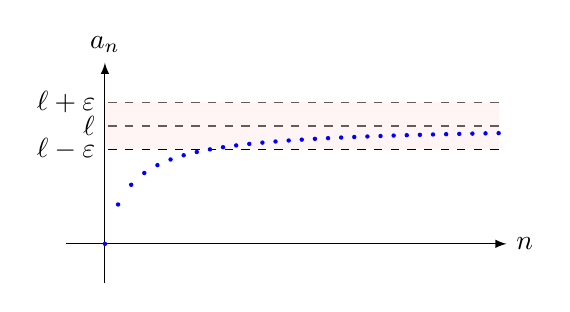
\begin{tikzpicture}
        \draw[-latex]   (-.5,0) -- (5.1,0) node[right] {$n$};
        \draw[-latex]   (0,-.5) -- (0,2.3) node[above] {$a_n$};
        \draw[thin,dashed] (5,1.8)--(0,1.8) node[left] () {$\ell+\varepsilon$};
        \draw[thick,dashed] (5,1.5)--(0,1.5) node[left] () {$\ell$};
        \draw[thin,dashed] (5,1.2)--(0,1.2) node[left] () {$\ell-\varepsilon$};
        \fill[red!10, opacity=0.4] (0,1.2) rectangle (5,1.8);
        \foreach \x in {0,...,30}
        \fill[blue] ({\x/6},{(2*\x+1)/(\x+2)-0.5}) circle(0.8pt); 
\end{tikzpicture}
\end{center}

\subsection{Rechenregeln für Grenzwerte}
Seien \(a, b\) zwei konvergente Folgen und \(c\) eine Konstante, so gelten folgende Rechenregeln:
\begin{align*}
    \lim_{n \to \infty} (c \cdot a_n) &= c \cdot \lim_{n \to \infty} a_n\\
    \lim\limits_{n \to \infty} (a_n \pm b_n) &= \lim\limits_{n \to \infty} a_n \pm \lim\limits_{n \to \infty} b_n\\
    \lim\limits_{n \to \infty} (a_n \cdot b_n) &= \lim\limits_{n \to \infty} a_n \cdot \lim\limits_{n \to \infty} b_n\\
    \lim\limits_{n \to \infty} \left(\frac{a_n}{b_n}\right) &= \frac{\lim\limits_{n \to \infty} a_n}{\lim\limits_{n \to \infty} b_n}, \quad \text{ falls } b \neq 0\\
\end{align*}

\subsection{Grenzwerte von Polynomen}
Sei \(p(n) = a_k n^k + a_{k-1} n^{k-1} + \ldots + a_1 n + a_0\) ein Polynom vom Grad \(k\) mit \(a_k \neq 0\). Dann gilt:
\[
\lim_{n \to \infty} p(n) = \begin{cases}
+\infty, & \text{falls } a_k > 0\\
-\infty, & \text{falls } a_k < 0
\end{cases}
\]

Sei \(p(n)\) und \(q(n)\) zwei Polynome vom Grad \(g_p\) bzw. \(g_q\) mit führenden Koeffizienten \(a_k\) bzw. \(b_m\). Dann gilt:
\[
\lim_{n \to \infty} \frac{p(n)}{q(n)} = \begin{cases}
0, & \text{falls } g_p < g_q\\
\frac{a_k}{b_m}, & \text{falls } g_p = g_q\\
+\infty, & \text{falls } g_p > g_q \text{ und } \frac{a_k}{b_m} > 0\\
-\infty, & \text{falls } g_p > g_q \text{ und } \frac{a_k}{b_m} < 0
\end{cases}
\]

\subsection{Wichtige Grenzwerte}
\begin{align*}
    \lim_{n \to \infty} \left(1 + \frac{1}{n}\right)^n &= e\\
    \lim_{n \to \infty} \sqrt[n]{a} &= 1, \quad a > 0\\
    \lim_{n \to \infty} q^n &= \begin{cases}
    0, & |q| < 1\\
    1, & q = 1\\
    +\infty, & q > 1\\
    \text{existiert nicht}, & q \le -1
    \end{cases}
\end{align*}

\subsection{Sandwich-Prinzip}
Seien \((a_n)\), \((b_n)\) und \((c_n)\) drei Folgen, so dass \(a_n \leq b_n \leq c_n\) für alle \(n\) ab einem gewissen Index \(n_0\). Falls \(\lim_{n \to \infty} a_n = \lim_{n \to \infty} c_n = L\) gilt, so konvergiert auch \((b_n)\) und es gilt \(\lim_{n \to \infty} b_n = L\).

\section{Kurvendiskussion}
\begin{itemize}
    \item Definitionsbereich
    \item Symmetrieeigenschaften (gerade, ungerade, periodisch)
    \item Schnittpunkte mit Achsen, Polstellen
    \item Randpunkte (Verhalten für \(x \to \pm \infty\))
    \item Extrempunkte
    \item Wendepunkte/Sattelpunkte
    \item Monotonieverhalten
\end{itemize}

\section{Optimierungsprobleme}
\begin{enumerate}
    \item Problem analysieren und Zielgröße festlegen
    \item Variablen und Nebenbedingungen definieren
    \item Zielfunktion aufstellen und ggf. auf eine Variable reduzieren
    \item Ableitung berechnen und kritische Punkte bestimmen
    \item Mit zweiter Ableitung bzw. Randwerten Optimum prüfen
    \item Ergebnis interpretieren
\end{enumerate}

\vfill

\rule{0.3\linewidth}{0.25pt}
\scriptsize

By Justin Iven Müller (2025)
\href{https://github.com/JustinIven/zhaw-cheatsheets}{github.com/JustinIven/zhaw-cheatsheets}


\end{multicols*}
\end{document}
